% !TEX root = /home/frank/School/thesis_text/thesis.tex


\chapter{High Level Synthesis}



A recurring theme in the literature is the relative difficulty of implementing an algorithm on an FPGA compared to conventional implementation techniques on CPU's and GPU's. Both development time and place-and-route take considerably more time compared to programming and compiling for more traditional architectures \cite{inta_chimera:_2012,tsoi_axel:_2010}. With an increase in the complexity required to perform a task also comes an increase in the difficulty of designing and debugging such a system. 
High level synthesis tools enable a user to specify the behavior of a system in a high level programming language and convert this description into usable hardware. Most tools use the C, C++ or systemC programming languages, however other programming languages such as the functional programming language Haskell \cite{baaij2010c}, the scripting language Python\cite{decaluwe2004myhdl} or Matlab M-code\cite{hdlcoder} have been used. These tools enable faster prototyping and implementation\cite{che_accelerating_2008}. These tools also enable programmers without a background in HDL design to benefit from the advantages of FPGA accelerators without facing the steep learning curve of learning a HDL such as VHDL or Verilog. For HDL designers these tools increase productivity by allowing the designer to describe the desired behavior using less code.\cite{casseau_c-_2005}. 
These tools enable to shift the focus from low-level implementation details to the development and improvement of the algorithm in a rapid prototyping fashion\cite{wakabayashi_c-based_2004}.
HLS tools have a long history dating back to the 1970's, but only recently have these tools matured enough to become adopted by industry. These tools present an interesting evolution and a possible paradigm shift in hardware design and prototyping\cite{cong_high-level_2011}.



\section{Riverside Optimizing Compiler for Configurable Computing} 
ROCCC is a C-to-VHDL compiler which focuses on FPGA based code acceleration. It implements a subset of the C language on which it performs loop analysis techniques to provide increasing throughput with less usage of area\cite{martin_high-level_2009}. The generated VHDL is independent from FPGA platforms and supports code reuse through the use of modules. 
ROCCC uses the streaming paradigm, in which data is represented by streams, a data format similar to the way arrays are stored in memory. These streams pass through a set of operations called kernels. This particular way of representing data makes it possible to express parallelism and is relatively easy mapped to the FPGA hardware. This paradigm removes the need for area-costly soft-core processors\cite{buyukkurt_impact_2006}.\\
This streaming paradigm is also what enables the platform independence of the ROCCC hardware. As long as the data is delivered to the system in the form of a stream it can be used.
Another important feature of ROCCC are the so-called smart buffers. These attempt to utilize the data-locality of certain applications to increase the performance. This is achieved through intelligent data reuse which minimizes the number of off-chip memory accesses. 

\section{Xilinx Vivado High-Level Synthesis Tool}
\label{sec:vivado_HLS}
Vivado High-Level Synthesis is part of the Xilinx Vivado design suite. It is the product of the acquisition of AutoESL and the re-branding of their AutoPilot High-Level Synthesis tool. Vivado represents the next evolution of Xilinx tools fitting in their vision of an \quotationmarks{all programmable world}.\\
Vivado HLS translates a subset of C, C++ or SystemC into VHDL or Verilog code. This is done through 2 types of synthesis: \emph{functional synthesis} and \emph{interface synthesis}. The functional synthesis synthesizes the functional statements into RTL statements spread over different clockcycles. The interface synthesis synthesizes the function parameters into ports with specific timing protocols. To do this the HLS tool extracts the control behavior and the datapath. The control is specified in the high level language by loops and conditional statements in the code. These get translated into state transitions in a finite state machine. The datapath is determined by unrolling all the loops and evaluating all the conditional statements. After the control behavior and datapath have been extracted, the actions that need to be taken are identified and scheduled to occur during in a state. This process takes into account the timing information and optimization directives to ensure optimal performance. After all the necessary actions are scheduled, the operations are bound to a specific hardware resource or core. The binding process influences the scheduling process so binding decisions are considered during scheduling. The directives allow the programmer to optimize for different parameters such as latency, area or initiation interval. The area is the number of resources a specific implementation uses. Latency is the number of clockcycles necessary to produce an output, and the initiation interval is the number of clockcycles that need to pass before a new input can be accepted. there are also directives that allow to constrain the latency of functions or loops and the area used, as well as specify of override dependencies in the code.\\
Vivado HLS supports a large subset of the C, C++ and SystemC languages, some constructs are not supported. Most notable are calls to the operating system, dynamic memory allocation and the C++ Standard Template Library. 
Vivado HLS has a number of features that can improve the productivity of a developer:

\paragraph{Verification}
Verifying the functionality of an algorithm and  the correct functioning of its implementation in hardware are important steps in the development process. Manually verifying the implementation through RTL simulation is a tedious and error-prone process. For this reason it is interesting to be able to automate these tests. Vivado HLS separates the verification into two discrete processes.\\ The first is the pre-synthesis validation, which does a functional validation of the high level code. The developer needs to develop a testbench, which provides an input for the function being verified, and compares the output of this function to a so called \emph{gold standard} which is the expected output.\\
The second verification process is the post synthesis verification. Vivado HLS provides an RTL implementation in VHDL of Verilog for which a testbench can be written. Vivado HLS also has the \texttt{cosim\_design} function which converts the high level testbench into a SystemC testbench. This low level testbench provides stimulus to the RTL code and compare the output to the \emph{gold standard}. This automation is possible when some requirements are satisfied:
\begin{itemize}
\item The top-level system needs to be synthesized with a supported control interface and the output ports need to have a valid signal.
\item Certain optimizations or combination of optimization on arrays in the function interface, either as an explicit array or hidden in a struct, are not supported.
\item The testbench needs to be self-checking, return 0 if the output is correct and a non-zero value when the output is incorrect.
\end{itemize}
Vivado HLS incorporates a simulation tool but also supports third-party simulators.

\paragraph{Data type conversions}
Whilst C-based data types have widths limited by byte boundaries, RTL buses don't have this constraint and can have an arbitrary width. Vivado HLS provides libraries for the supported programming languages that allow to specify the desired width between 1 and 1024 for integers in C and C++. The \texttt{\_\_SYNTHESIS\_\_} macro allows to retain the original declarations for backwards compatibility and reference purposes.\\ Vivado HLS also has libraries for fixed-point types. Fixed point operations are often preferred by HDL designers because of the reduced resource consumption. These libraries also ensure that the high-level and RTL behavior remain the same. This allows the designer to use the high-level simulations to study the effects of the reduced precision compared to floating-point representations. These fixed point data types are available in C++ and SystemC.\\
Floating point arithmetic is supported, however not all operations are supported. 

\paragraph{Interface Synthesis}
Vivado HLS supports a number of different interfaces that can be used to convert the function arguments into RTL ports. These standard interfaces can range from control signals to elaborate handshaking protocols and memory interfaces. Vivado HLS also supports a number of bus interfaces. These differ form the standard interfaces in that they only get added to the system during the export to RTL. The supported bus interfaces are:
\begin{itemize}
	\item AXI4-Lite Slave
	\item AXI4 Master
	\item AXI4 Stream
\end{itemize}

These bus interfaces sit ``on top of'' the RTL interfaces, and only certain RTL interfaces can be connected to certain bus interfaces.

\paragraph{Optimizations}
Vivado HLS supports a large number of optimizations on the function, loop and array level.

The available function optimizations are

\begin{itemize}
	
	\item 	\textbf{Inline} The \emph{inline} directive places the function in-line, removing all hierarchy. This removes the cycles needed to enter and leave the function.
	
	\item 	\textbf{Instantiate}  By default functions remain separate hierarchical blocks in the RTL and all the instantiations use the same RTL implementation. The \emph{instantiate} directive lets the compiler create a separate,
	unique and optimized implementation for each instance of the function. 
	
	\item 	\textbf{Dataflow} The \emph{dataflow} directive will have the compiler attempt to execute each RTL function block at the same time. If data dependencies prevent this the interval will be modified until the dependencies are satisfied. This effectively pipelines the communication between the functions. The channels can be configured to be ping-pong or FIFO buffers. 
	
	\item 	\textbf{Pipeline} Whereas the \emph{dataflow} directive pipelines the communication between different functions, the \emph{pipeline} directive pipelines the operations within a function. This allows these operations to happen concurrently. As with dataflow pipelining data dependencies can prevent pipelining. The solution is to increase the initiation interval until the dependencies are satisfied.
	
	\item 	\textbf{Latency} The latency of a function can be specified using the \emph{latency} directive. The synthesis process tries to stay within the constraints set by the directive and allows timing violations in doing so. If the system cannot satisfy the constraints they are automatically relaxed. After synthesis the constraint report details whether all constraints have been satisfied.
\end{itemize}

On the loop level a number of optimizations are available. The \emph{dataflow}, \emph{pipeline} and \emph{latency} optimizations are also available for loops and have functionality comparable to the aforementioned optimizations for functions. The other ones are:

\begin{itemize}

	\item 	\textbf{Unrolling} The default behavior for Vivado HLS is that all loops remain rolled. This means that every iteration of the loop uses the same hardware. The \emph{unroll} directive allows the designer to partially or completely split the iterations of a loop into separate entities. Multiple iterations can then be executed concurrently. Unrolling a loop presents a trade-off between resource consumption and performance. 

	\item 	\textbf{Merging} A loop takes one cycle to enter and one cycle to exit from. If there are consecutive loops in the design these states are unnecessary. The \emph{merge} optimization combines these consecutive loops into one loop, no longer requiring multiple cycles to enter and exit a loop.

	\item 	\textbf{Flattening} This optimization is similar to the \emph{merging} optimization, but applied to nested loops instead of consecutive loops. The nested loops are combined into one loop removing the need for extra clockcycles to enter and exit the innermost loop. When loops are nested the outermost loop cannot be pipelined. \emph{Flattening} prevents this.

	\item 	\textbf{Dependence} The compiler tries to identify dependencies between calculations or resources. Sometimes this automatic identification of dependencies is too conservative because the compiler does not have the necessary information. For this reason the \emph{dependence} directive exists, allowing the programmer to explicitly state that there are or aren't dependencies for a certain variable. There are two types of dependence:
	\begin{description}
		\item[Inter] The dependence is between different iterations of the same loop. If the dependence is set to `false', the compiler will not prevent the loop from being unrolled.
		\item[Intra] The dependence is inside the iteration. If the dependence is set to be `false' the compiler will attempt to reorder the operations for the most optimal performance.
	\end{description}

	\item 	\textbf{Tripcount} HLS tries to determine the maximum possible number of iterations that a loop can perform during the execution. The compiler cannot determine the actual maximum iteration of a loop. The \emph{tripcount} optimization provides this data to the compiler, so as to ensures that the synthesis report will contain valid figures for throughput and latency. This optimization does not influence the synthesis process and only exists to provide metadata to the compiler. 
\end{itemize}

Finally there are also optimizations that determine the memory architecture of the design. The way memory accesses are implemented are an important factor influencing the performance of an IP-Core. Using buffers is a way to increase the computational intensity, thereby decreasing the load on the memory 
In \emph{High Level} programming languages memory gets abstracted to variables and array's. These abstractions need to be translated into something that can be implemented in hardware. For FPGA's this means choosing between \emph{block ram} or registers. The process of translating the memory constructs into the most fitting type of physical memory is controlled by the HLS compiler. This process can be influenced by using directives or pragma's. Especially the manner in which arrays are translated into hardware is of importance. For this purpose a couple of directives are available.\\

\begin{itemize}

	\item 	\textbf{Resource} The default behavior of Vivado HLS is to select the memory to be used. The \emph{resource} optimization allows the designer to override this decision and specify which type of memory needs to be used to implement an array. 

	\item 	\textbf{Array Mapping} The RAMs available in an FPGA have pre-defined sizes. Having to store many arrays each in their own RAM increases the resource consumption. The \emph{array map} directive allows the designer to map multiple arrays onto one RAM reducing the resource consumption. There are two types of mapping. Horizontal mapping concatenates the original arrays to create an implementation using a single array with more elements. Vertical mapping concatenates the words in the array to create an implementation that uses a single array with a larger bit-width. 
	
	\item 	\textbf{Array\_Partition} The \emph{array partition} optimization performs the opposite of the \emph{array mapping} optimization. It splits a large array into a number of smaller arrays which can each be mapped onto a different RAM. This allows for multiple consecutive reads or writes to memory. There are three possible ways to partition. Block partitions separate the array into a number equally sized blocks containing consecutive elements of the original array. Cyclic partitions split the array into a number of equally sized blocks with the elements of the original array interleaved. Complete partitioning separates the array and stores the individual elements in registers. The number of blocks in which the arrays are split can be specified by a factor.

	\item 	\textbf{Array\_Reshape} The \emph{array reshape} optimization combines array partitioning with vertical mapping. It takes elements from one dimension in the original array and maps them to a single element with a larger bitwidth in the reshaped array. 

\end{itemize}

\paragraph{Pragmas and directives}
The aforementioned optimizations can be applied to a design using 2 methods. The first one is by embedding pragmas in the source code. In C-style languages pragmas are typically specified as preprocessor directives. These directives provide the compiler with meta-information concerning the way the code should be converted to machine code. Vivado HLS has its specific pragmas who serve the same function.
The second method is by using the directives file, a TCL script that specifies the optimizations that need to be applied. The optimizations that can be applied are the same for both methods, which makes the two possibilities seem redundant. There are however subtle differences in the usage.\\
Vivado HLS has a feature called a \emph{solution}. These solutions allow a designer to quickly do design space exploration. This is achieved by applying many different combinations of directives in each solution. The designer can then measure the impact and compare the performance of different solutions. This can only be achieved by using the directives file as the code is shared between solutions. Pragmas are useful when the directives need to remain the same irrespective of the solution. This is for example the case when using libraries.

\paragraph{Synthesis report \& Analysis perspective}
Vivado HLS generates a report after the synthesis has finished. This \emph{synthesis report} contains, next to some general information, performance estimates for the timing, latency an resource consumption. The timing information comprises an estimate of the smallest attainable clock period, the uncertainty and whether this estimate satisfies the target clock period. The latency information comprises an estimate of the function's latency as well as the initiation interval for the block and all sub-blocks. the utilization estimates detail the expected utilization of resources present in the FPGA such as LUTs or DSP48s. A more detailed view is also given, showing the estimates of the resource consumption of different cores.\\
Another feature of Vivado HLS that can help in estimating the performance of an implementation is the \emph{analysis perspective}. The analysis perspective provides the designer with a graphical representation of the design's performance and resource usage, as well as the scheduling of the different operations. An example of the schedule viewer pane is given in figure \ref{img:schedule_viewer}.

\begin{figure}[H]
\centering
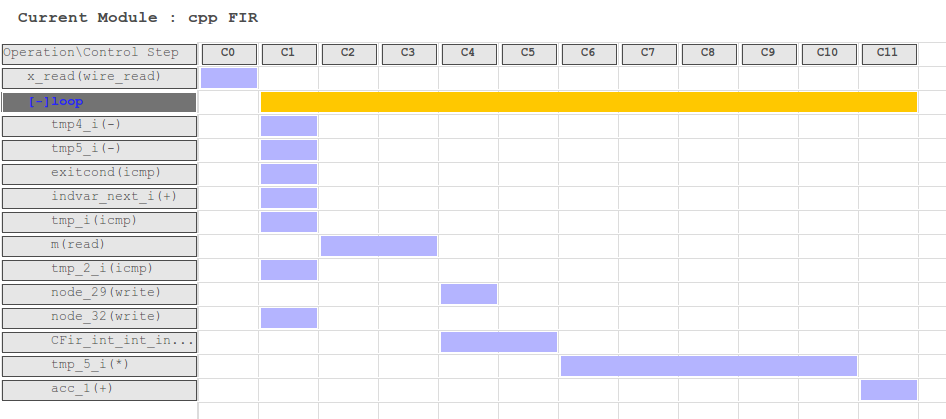
\includegraphics[scale=0.4]{./images/schedule_viewer_example.png}
\caption{Example of the Schedule Viewer Pane}
\label{img:schedule_viewer}
\end{figure}

The left column details the resources. Loops are marked in yellow and operations are marked in purple. The numbered columns each represent a state in the FSM. This allows the designer to see where resources are being used concurrently and where there are dependency issues preventing this. The schedule viewer also has a ``Goto Source'' command, which jumps form the selected operation to the corresponding line in the high level source code. Using this functionality the designer can link the high level code to the execution of the hardware.

\paragraph{Exporting} Vivado HLS is part of Xilinx' Vivado toolchain and is backwards compatible with its ISE toolchain. This tight integration is most visible in the available export options in Vivado HLS. Dependent on the target technology and available license it can export to formats supported by the Vivado IP-catalog, Xilinx System Generator and EDK PCore. If the core is configured to use the AXI protocol the wrappers will be added in this step. The AXI wrappers are not part of the VHDL or Verilog implementation.
\\\\
Vivado HLS version 2013.2 was used for this thesis. 

